\title{Memoria: Procesadores de Lenguaje - Lenguaje Tiny}
\author{Burgos Sosa, Rodrigo \and Cassin, Gina Andrea \and Estebán Velasco, Luis \and Rabbia, Santiago Elias}
\date{Curso 2024}

% Preamble
\documentclass[11pt]{article}

% Packages
\usepackage{amsmath}
\usepackage{graphicx}
\graphicspath{ {/} }

% Document
\begin{document}
\maketitle
\thispagestyle{empty}
    \begin{center}
        \large Grupo G03
    \end{center}

    \newpage

    \section{Introducción}
        En el siguiente documento se expondrá una memoria sobre el desarrollo de analizadores léxicos aplicado sobre dos lenguajes de programación, Tiny y Tiny(0) - un subconjunto de Tiny.
        Se presentará una descripción de las clases léxicas y una especificación formal de ambos lenguajes, y un analizador léxico para Tiny(0).

    \section{Análisis léxico}
    La función de un analizador léxico es segmentar el programa de entrada en una secuencia de componentes léxicos o tokens. La primera fase en el desarrollo del analizador léxico (y la fase
más importante) es llevar a cabo su especificación léxica. Esto se llevará a cabo a continuación:

    \subsection{Tiny(0)}
    \subsubsection{Clases léxicas}
        A continuación se presentan las clases léxicas del lenguaje Tiny(0):
        \subsubsection*{Clases léxicas}
        \begin{itemize}
            \item \textbf{Identificador (variable)}: Comienzan necesariamente por una letra o subrayado (\_), seguida de una secuencia de cero o más letras, dígitos, o subrayado (\_).
            \item \textbf{Una clase léxica por cada tipo de variable}:
                \begin{itemize}
                    \item \textbf{int}: representa los números enteros.
                    \item \textbf{real}: representa los números reales.
                    \item \textbf{bool}: representa los valores booleanos (true o false).
                \end{itemize}
            \item \textbf{Literal entero}
            \item \textbf{Literal real}
            \item \textbf{Literal booleano}
            \item \textbf{Una clase léxica por cada operador aritmético}:
                \begin{itemize}
                    \item \textbf{+}: suma.
                    \item \textbf{-}: resta.
                    \item \textbf{*}: multiplicación.
                    \item \textbf{/}: división.
                \end{itemize}
            \item \textbf{Una clase léxica por cada operador lógico}:
                \begin{itemize}
                    \item \textbf{and}: conjunción.
                    \item \textbf{or}: disyunción.
                    \item \textbf{not}: negación.
                \end{itemize}
            \item \textbf{Una clase léxica por cada operador relacional}:
                \begin{itemize}
                    \item \textbf{\textless}: menor que.
                    \item \textbf{\textgreater}: mayor que.
                    \item \textbf{\textless=}: menor o igual que.
                    \item \textbf{\textgreater=}: mayor o igual que.
                    \item \textbf{==}: igual que.
                    \item \textbf{!=}: distinto que.
                \end{itemize}
            \item \textbf{Una clase léxica por cada símbolo de puntuación}:
                \begin{itemize}
                    \item \textbf{(}: paréntesis izquierdo. Sirve para asociatividad.
                    \item \textbf{)}: paréntesis derecho. Sirve para asociatividad.
                    \item \textbf{;}: punto y coma. Sirve para separar declaraciones en la seccion de declaraciones, o separar instrucciones en la seccion de instrucciones. 
                    \item \textbf{.}: punto. Para los decimales.
                    \item \textbf{\{}: llave izquierda. Indica el inicio de un bloque de código.
                    \item \textbf{\}}: llave derecha. Indica el fin de un bloque de código.
                    \item \textbf{$\&\&$}: doble signo et. Indica el fin de declaraciones.
                \end{itemize}
            \item \textbf{Operador de asignación}: =
            \item \textbf{Operador de evaluación}: @
        \end{itemize}
        \subsubsection*{Cadenas ignorables}
        \begin{itemize}
            \item \textbf{Espacios en blanco}.
            \item \textbf{Retroceso}: \textbackslash b
            \item \textbf{Tabulador}: \textbackslash t
            \item \textbf{Retorno de carro}: \textbackslash r
            \item \textbf{Salto de línea}: \textbackslash n
            \item \textbf{Comentarios}: comienzan con \#\# y terminan con un salto de línea.
        \end{itemize}
    \subsubsection{Especificación formal}
        \subsubsection*{Definiciones auxiliares}
        \begin{itemize}
            \item \textbf{letra }$\equiv$ [a-z,A-Z]
            \item \textbf{digito }$\equiv$ [0-9]
            \item \textbf{digitoSinCero }$\equiv$ [1-9]
            \item \textbf{parteEntera }$\equiv$ (\{digitoSinCero\} \{digito\}*) \textbar\ 0
            \item \textbf{parteDecimal }$\equiv$ (\{digito\}* \{digitoSinCero\}) \textbar\ 0
        \end{itemize}
        \subsubsection*{Definiciones léxicas}
        \begin{itemize}
            \item \textbf{suma }$\equiv$ \textbackslash+
            \item \textbf{resta }$\equiv$ \textbackslash-
            \item \textbf{mul }$\equiv$ \textbackslash*
            \item \textbf{div }$\equiv$ /
            \item \textbf{parentesisAbrir }$\equiv$ \textbackslash(
            \item \textbf{parentesisCerrar }$\equiv$ \textbackslash)
            \item \textbf{abrirBloque }$\equiv$ \textbackslash\{
            \item \textbf{cerrarBloque }$\equiv$ \textbackslash\}
            \item \textbf{separadorDeclaraciones }$\equiv$ ;
            \item \textbf{finDeclaraciones }$\equiv \&\& $
            \item \textbf{asignacion }$\equiv$ \textbackslash=
            \item \textbf{menor }$\equiv$ \textless
            \item \textbf{mayor }$\equiv$ \textgreater
            \item \textbf{menorIgual }$\equiv$ \textless\textbackslash=
            \item \textbf{mayorIgual }$\equiv$ \textgreater\textbackslash=
            \item \textbf{igual }$\equiv$ \textbackslash=\textbackslash=
            \item \textbf{no igual }$\equiv$ !\textbackslash=
            \item \textbf{and }$\equiv$ (a \textbar\ A)(n \textbar\ N)(d \textbar\ D)
            \item \textbf{or }$\equiv$ (o \textbar\ O)(r \textbar\ R)
            \item \textbf{not }$\equiv$ (n \textbar\ N)(o \textbar\ O)(t \textbar\ T)
            \item \textbf{true }$\equiv$ (t \textbar\ T)(r \textbar\ R)(u \textbar\ U)(e \textbar\ E)
            \item \textbf{false }$\equiv$ (f \textbar\ F)(a \textbar\ A)(l \textbar\ L)(s \textbar\ S)(e \textbar\ E)
            \item \textbf{tipo entero }$\equiv$ int
            \item \textbf{tipo real }$\equiv$ real
            \item \textbf{tipo booleano }$\equiv$ bool
            \item \textbf{eval }$\equiv$ @
            \item \textbf{punto }$\equiv$ \textbackslash.
            \item \textbf{identificador }$\equiv$ (\{letra\} \textbar\ \_) (\{letra\} \textbar\ \{dígito\} \textbar\ \_ )*
            \item \textbf{literalEntero }$\equiv$ ( \textbackslash + \textbar\ \textbackslash - )? \{parteEntera\}
            \item \textbf{literalReal }  $\equiv$ \{literalEntero\}((\textbackslash.\{parteDecimal\})((e \textbar\ E)\{literalEntero\})) \textbar\ (\textbackslash.\{parteDecimal\}) \textbar\ ((e \textbar\ E)\{literalEntero\})
        \end{itemize}
        \subsubsection*{Definiciones cadenas ignorables}
        \begin{itemize}
            \item \textbf{separador }$\equiv$ [ ,\textbackslash t,\textbackslash r,\textbackslash b,\textbackslash n]
            \item \textbf{comentario }$\equiv$ \#\#([\^{}\textbackslash n, EOF])*
        \end{itemize}
    \subsubsection{Diagrama de transiciones}
        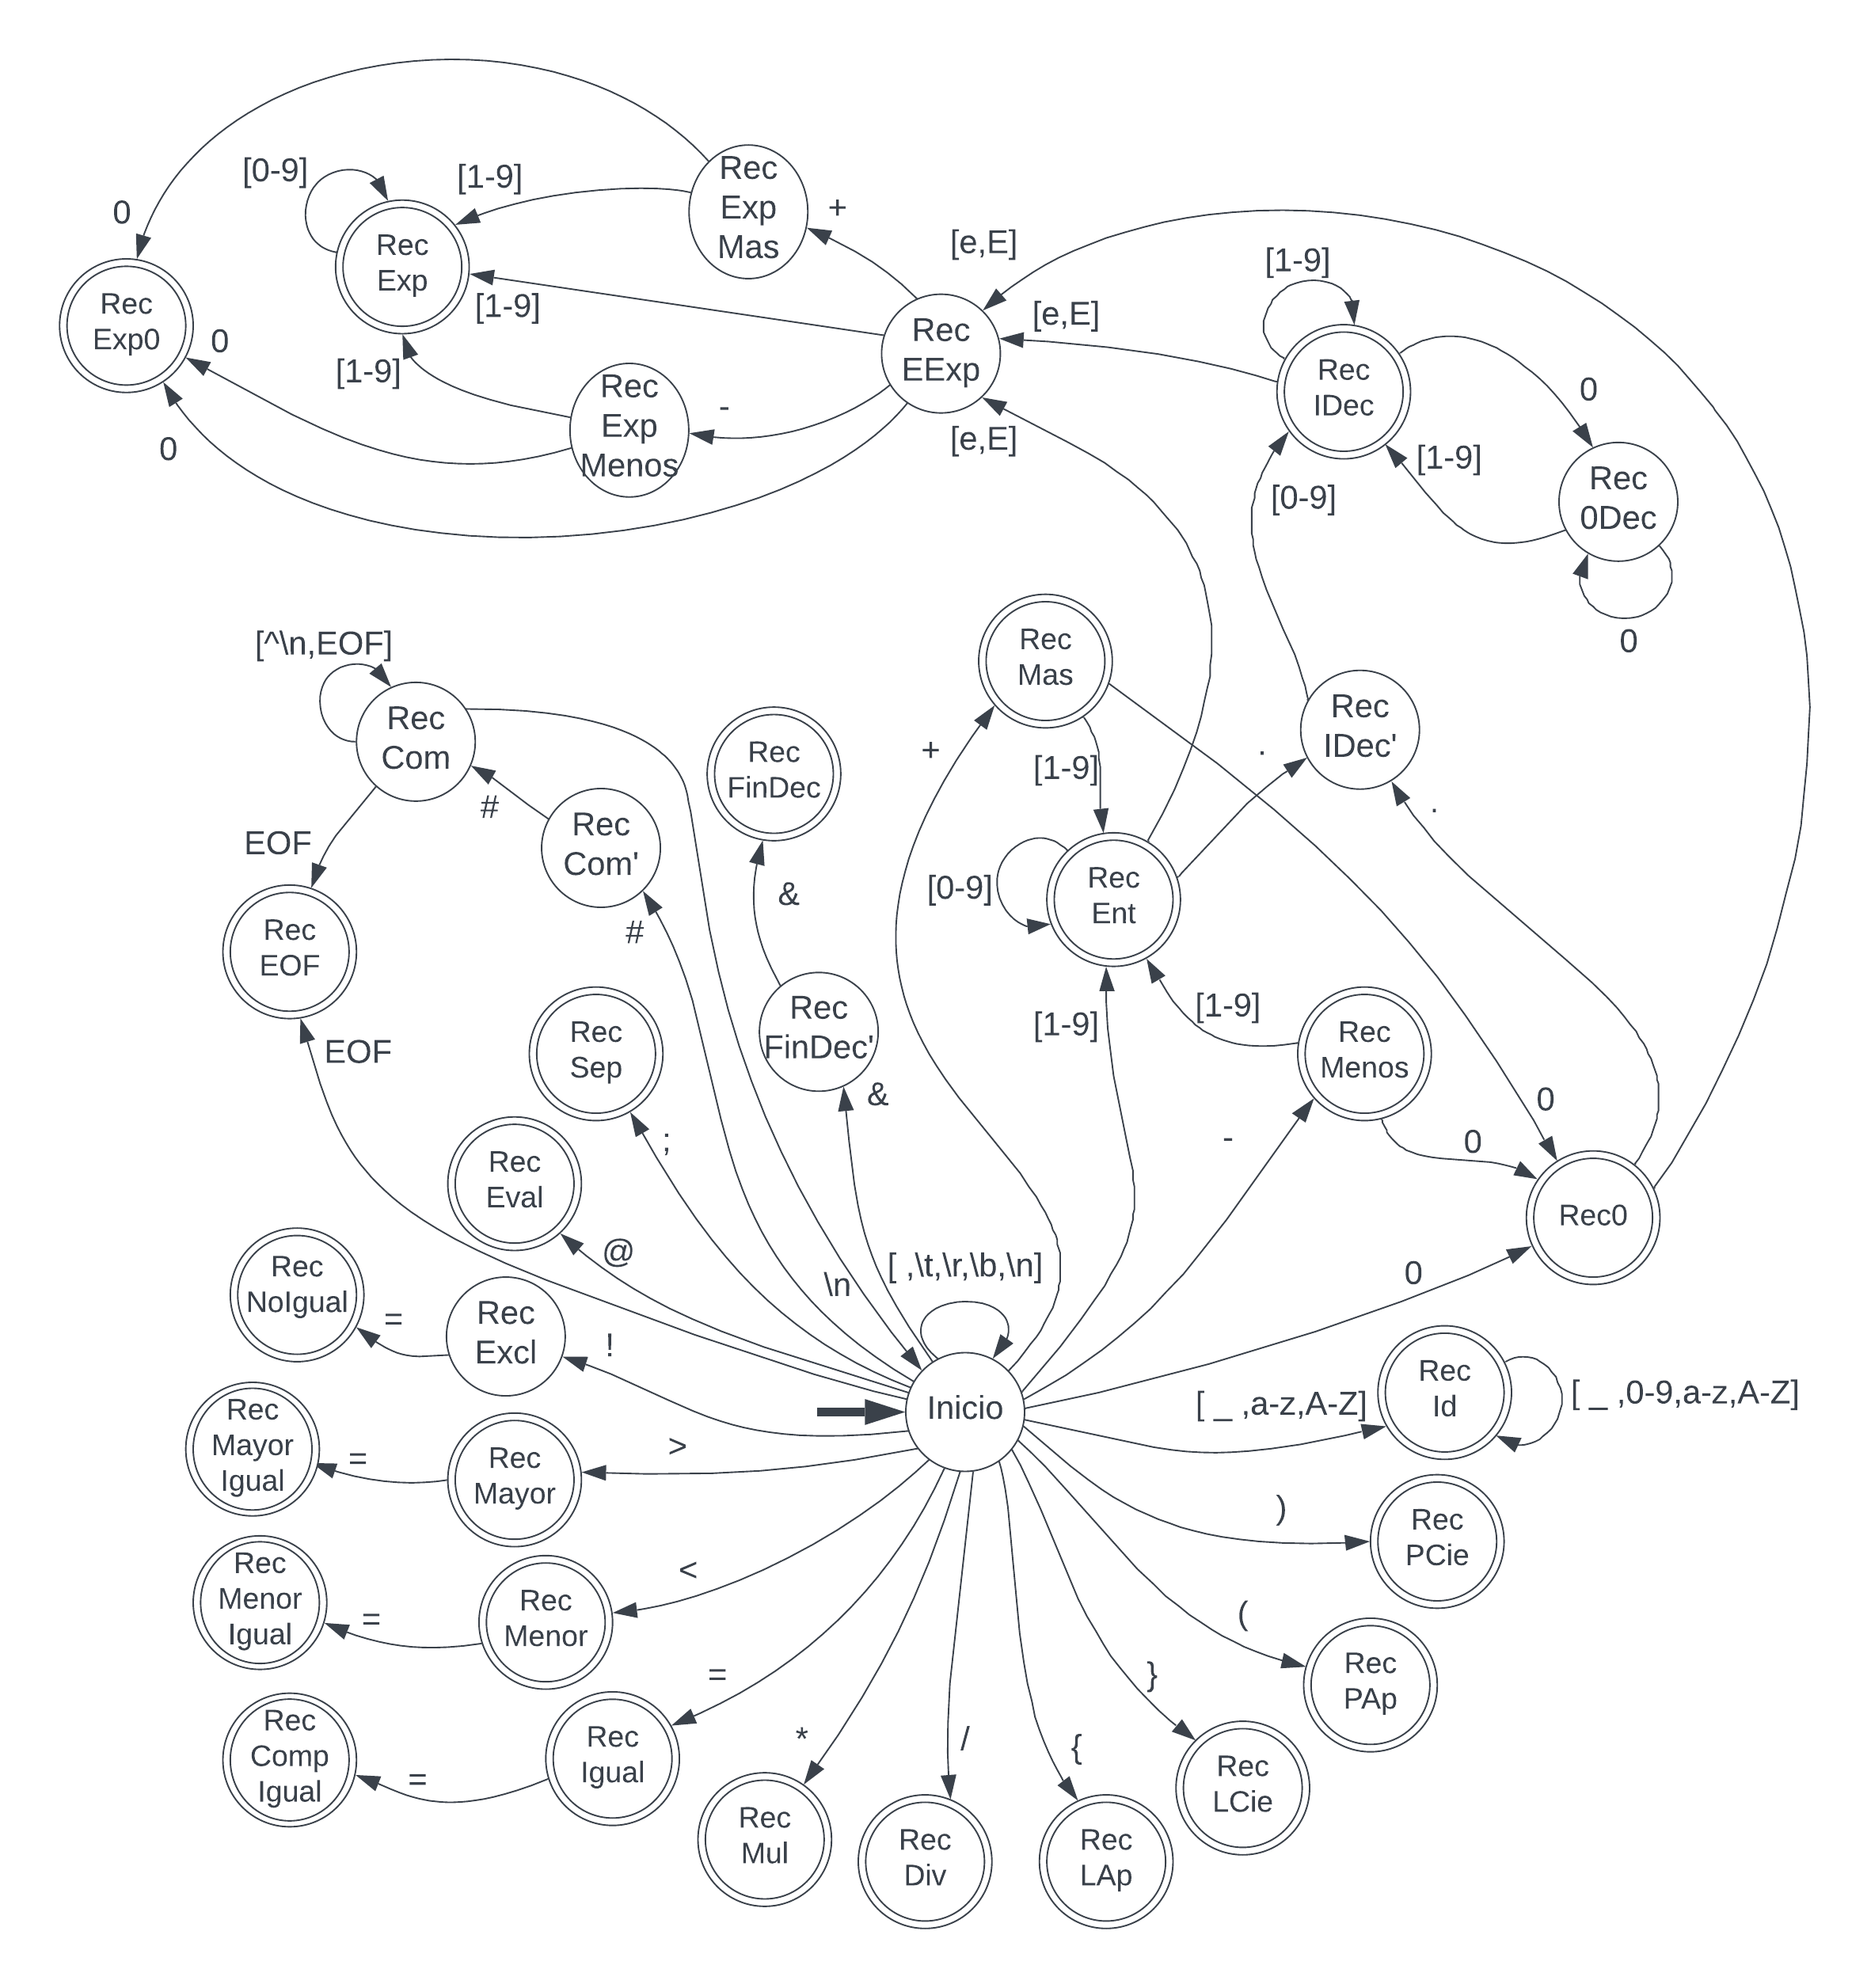
\includegraphics[scale=0.2]{tiny0}
    \subsection{Tiny}
        \subsubsection{Clases léxicas}
        A continuación se presentan las clases léxicas del lenguaje Tiny:
        \subsubsection*{Clases léxicas}
        \begin{itemize}
            \item \textbf{Identificador (variable)}: Comienzan necesariamente por una letra o subrayado (\_), seguida de una secuencia de cero o más letras, dígitos, o subrayado (\_).
            \item \textbf{Una clase léxica por cada tipo de variable}:
            \begin{itemize}
                \item \textbf{int}: representa los números enteros.
                \item \textbf{real}: representa los números reales.
                \item \textbf{bool}: representa los valores booleanos (true o false).
                \item \textbf{string}: representa las cadenas de caracteres.
                \item \textbf{array}: representa los arreglos.
            \end{itemize}
            \item \textbf{Literal entero}
            \item \textbf{Literal real}
            \item \textbf{Literal booleano}
            \item \textbf{Literal cadena}
            \item \textbf{Una clase léxica por cada operador aritmético}:
            \begin{itemize}
                \item \textbf{+}: suma.
                \item \textbf{-}: resta.
                \item \textbf{*}: multiplicación.
                \item \textbf{/}: división.
            \end{itemize}
            \item \textbf{Una clase léxica por cada operador lógico}:
            \begin{itemize}
                \item \textbf{and}: conjunción.
                \item \textbf{or}: disyunción.
                \item \textbf{not}: negación.
            \end{itemize}
            \item \textbf{Una clase léxica por cada operador relacional}:
            \begin{itemize}
                \item \textbf{\textless}: menor que.
                \item \textbf{\textgreater}: mayor que.
                \item \textbf{\textless=}: menor o igual que.
                \item \textbf{\textgreater=}: mayor o igual que.
                \item \textbf{==}: igual que.
                \item \textbf{!=}: distinto que.
            \end{itemize}
            \item \textbf{Una clase léxica por cada símbolo de puntuación}:
            \begin{itemize}
                \item \textbf{(}: paréntesis izquierdo. Sirve para asociatividad. También indica el inicio de una lista de parámetros cuando se definen procedimientos y el inicio de argumentos cuando se llama una función.
                \item \textbf{)}: paréntesis derecho. Sirve para asociatividad. También indica el fin de una lista de parámetros cuando se definen procedimientos y el fin de argumentos cuando se llama una función.
                \item \textbf{;}: punto y coma. Sirve para separar declaraciones en la sección de declaraciones, o separar instrucciones en la sección de instrucciones.
                \item \textbf{,}: coma. Separa los campos dentro de la definición de un struct, los parámetros en la definición de un procedimiento, y los argumentos en la llamada a una función.
                \item \textbf{.}: punto. Para los decimales, y es un operador de "acceso a registro".
                \item \textbf{\{}: llave izquierda. Indica el inicio de un bloque de código. También indica el inicio de la definición de un struct.
                \item \textbf{\}}: llave derecha. Indica el fin de un bloque de código. También indica el fin de la definición de un struct.
                \item \textbf{$\&$}: signo et simple. Indica que un parámetro de un procedimiento se pasa por referencia.
                \item \textbf{$\&\&$}: doble signo et. Indica el fin de declaraciones.
                \item \textbf{[}: corchete izquierdo. Operador de indexación.
                \item \textbf{]}: corchete derecho. Operador de indexación.
                \item \textbf{\%}: operador módulo.
                \item \textbf{\^{}}: acento circunflejo. Se usa para definir un puntero. También es el operador de indirección.
            \end{itemize}
            \item \textbf{Operador de asignación}: =
            \item \textbf{Operador de evaluación}: @
            \item \textbf{Una clase léxica por cada palabra reservada}:
                \begin{itemize}
                    \item \textbf{null}: representa el valor nulo.
                    \item \textbf{proc}: palabra reservada para definir un procedimiento.
                    \item \textbf{if}: palabra reservada para definir una condición.
                    \item \textbf{else}: palabra reservada para definir una condición alternativa.
                    \item \textbf{while}: palabra reservada para definir un bucle.
                    \item \textbf{struct}: palabra reservada para definir una estructura.
                    \item \textbf{new}: palabra reservada para instrucción de reserva de memoria.
                    \item \textbf{delete}: palabra reservada para instrucción de liberación de memoria.
                    \item \textbf{read}: palabra reservada para instrucción de lectura.
                    \item \textbf{write}: palabra reservada para instrucción de escritura.
                    \item \textbf{nl}: palabra reservada para instrucción de nueva linea.
                    \item \textbf{type}: palabra reservada para declaración de tipo.
                    \item \textbf{call}: palabra reservada para instrucción de invocación a procedimiento.
                \end{itemize}
        \end{itemize}
        \subsubsection*{Cadenas ignorables}
        \begin{itemize}
            \item \textbf{Espacios en blanco}.
            \item \textbf{Retroceso}: \textbackslash b
            \item \textbf{Tabulador}: \textbackslash t
            \item \textbf{Retorno de carro}: \textbackslash r
            \item \textbf{Salto de línea}: \textbackslash n
            \item \textbf{Comentarios}: comienzan con \#\# y terminan con un salto de línea.
        \end{itemize}
        \subsubsection{Especificación formal}
        \subsubsection*{Definiciones auxiliares}
        \begin{itemize}
            \item \textbf{letra }$\equiv$ [a-z,A-Z]
            \item \textbf{digito }$\equiv$ [0-9]
            \item \textbf{digitoSinCero }$\equiv$ [1-9]
            \item \textbf{parteEntera }$\equiv$ (\{digitoSinCero\} \{digito\}*) \textbar\ 0
            \item \textbf{parteDecimal }$\equiv$ (\{digito\}* \{digitoSinCero\}) \textbar\ 0
        \end{itemize}
        \subsubsection*{Definiciones léxicas}
        \begin{itemize}
            \item \textbf{suma }$\equiv$ \textbackslash+
            \item \textbf{resta }$\equiv$ \textbackslash-
            \item \textbf{mul }$\equiv$ \textbackslash*
            \item \textbf{div }$\equiv$ /
            \item \textbf{parentesisAbrir }$\equiv$ \textbackslash(
            \item \textbf{parentesisCerrar }$\equiv$ \textbackslash)
            \item \textbf{abrirBloque }$\equiv$ \textbackslash\{
            \item \textbf{cerrarBloque }$\equiv$ \textbackslash\}
            \item \textbf{tamañoAbrir  }$\equiv$ [
            \item \textbf{tamañoCerrar }$\equiv$ ]
            \item \textbf{finDeclaraciones }$\equiv \&\& $
            \item \textbf{asignacion }$\equiv$ \textbackslash=
            \item \textbf{menor }$\equiv$ \textless
            \item \textbf{mayor }$\equiv$ \textgreater
            \item \textbf{menorIgual }$\equiv$ \textless\textbackslash=
            \item \textbf{mayorIgual }$\equiv$ \textgreater\textbackslash=
            \item \textbf{igual }$\equiv$ \textbackslash=\textbackslash=
            \item \textbf{no igual }$\equiv$ !\textbackslash=
            \item \textbf{and }$\equiv$ (a \textbar\ A)(n \textbar\ N)(d \textbar\ D)
            \item \textbf{or }$\equiv$ (o \textbar\ O)(r \textbar\ R)
            \item \textbf{not }$\equiv$ (n \textbar\ N)(o \textbar\ O)(t \textbar\ T)
            \item \textbf{true }$\equiv$ (t \textbar\ T)(r \textbar\ R)(u \textbar\ U)(e \textbar\ E)
            \item \textbf{false }$\equiv$ (f \textbar\ F)(a \textbar\ A)(l \textbar\ L)(s \textbar\ S)(e \textbar\ E)
            \item \textbf{modulo }$\equiv$ \%
            \item \textbf{puntero }$\equiv$ \^{}
            \item \textbf{bitwiseAnd }$\equiv$ $\&$
            \item \textbf{tipo entero }$\equiv$ int
            \item \textbf{tipo real }$\equiv$ real
            \item \textbf{tipo booleano }$\equiv$ bool
            \item \textbf{tipo string }$\equiv$ string
            \item \textbf{tipo array }$\equiv$ array
            \item \textbf{null }$\equiv$ (n \textbar\ N)(u \textbar\ U)(l \textbar\ L)(l \textbar\ L)
            \item \textbf{procedimiento }$\equiv$ (p \textbar\ P)(r \textbar\ R)(o \textbar\ O)(c \textbar\ C)
            \item \textbf{if }$\equiv$ (i \textbar\ I)(f \textbar\ F)
            \item \textbf{else }$\equiv$ (e \textbar\ E)(l \textbar\ L)(s \textbar\ S)(e \textbar\ E)
            \item \textbf{while }$\equiv$ (w \textbar\ W)(h \textbar\ H)(i \textbar\ I)(l \textbar\ L)(e \textbar\ E)
            \item \textbf{struct }$\equiv$ (s \textbar\ S)(t \textbar\ T)(r \textbar\ R)(u \textbar\ U)(c \textbar\ C)(t \textbar\ T)
            \item \textbf{new }$\equiv$ (n \textbar\ N)(e \textbar\ E)(w \textbar\ W)
            \item \textbf{delete }$\equiv$ (d \textbar\ D)(e \textbar\ E)(l \textbar\ L)(e \textbar\ E)(t \textbar\ T)(e \textbar\ E)
            \item \textbf{read }$\equiv$ (r \textbar\ R)(e \textbar\ E)(a \textbar\ A)(d \textbar\ D)
            \item \textbf{write }$\equiv$ (w \textbar\ W)(r \textbar\ R)(i \textbar\ I)(t \textbar\ T)(e \textbar\ E)
            \item \textbf{nl }$\equiv$ (n \textbar\ N)(l \textbar\ L)
            \item \textbf{type }$\equiv$ (t \textbar\ T)(y \textbar\ Y)(p \textbar\ P)(e \textbar\ E)
            \item \textbf{call }$\equiv$ (c \textbar\ C)(a \textbar\ A)(l \textbar\ L)(l \textbar\ L)
            \item \textbf{eval }$\equiv$ @
            \item \textbf{punto }$\equiv$ \textbackslash.
            \item \textbf{identificador }$\equiv$ (\{letra\} \textbar\ \_) (\{letra\} \textbar\ \{dígito\} \textbar\ \_ )*
            \item \textbf{literalEntero }$\equiv$ ( \textbackslash + \textbar\ \textbackslash - )? \{parteEntera\}
            \item \textbf{literalReal }  $\equiv$ \{literalEntero\}((\textbackslash.\{parteDecimal\})((e \textbar\ E)\{literalEntero\})) \textbar\ (\textbackslash.\{parteDecimal\}) \textbar\ ((e \textbar\ E)\{literalEntero\})
        \end{itemize}
        \subsubsection*{Definiciones cadenas ignorables}
        \begin{itemize}
            \item \textbf{separador }$\equiv$ [ ,\textbackslash t,\textbackslash r,\textbackslash b,\textbackslash n]
            \item \textbf{comentario }$\equiv$ \#\#([\^{}\textbackslash n, EOF])*
        \end{itemize}


\end{document}